\documentclass[10pt]{article}
\usepackage[margin=0.72in]{geometry}
\usepackage{graphicx}
\usepackage{booktabs}
\usepackage{hyperref}
\title{Streamed D5 certificate custody qualification}
\author{Semaev quotient-lift evidence packet}
\date{1 November 2026}
\begin{document}
\maketitle
\noindent The bounded exporter, AWS CLI stream upload, full S3 readback, and original independent checker completed one native small-system control without a local output certificate. The downloaded bytes were hashed while being fed to the checker. This is a transport and checker qualification, not a high-memory n51 trial.

\begin{center}
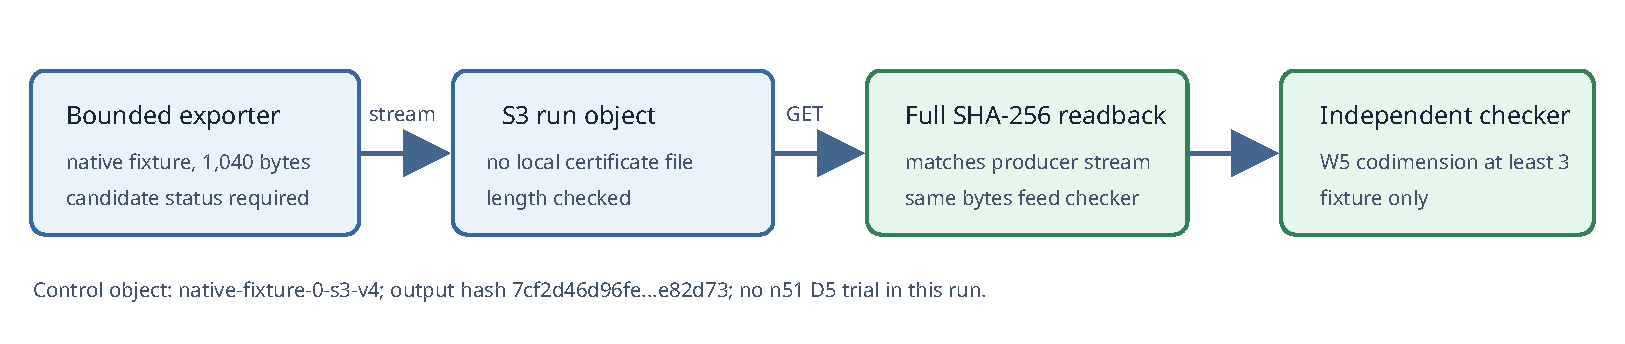
\includegraphics[width=\textwidth]{pipeline.pdf}
\end{center}

\begin{center}
\begin{tabular}{ll}
\toprule
Control output & 1,040-byte certificate \\
Original and readback SHA-256 & \texttt{7cf2d46d96fe...e82d73} \\
Independent checker & $1\notin W_5(F)$; codimension at least 3 \\
Local controls & 4 passed; changed input/readback and failed producer rejected \\
\bottomrule
\end{tabular}
\end{center}

\noindent The object is stored at:
\begin{flushleft}\small\texttt{s3://setec-astronomy-artifacts/validation/}\\
\texttt{semaev-d5-stream-custody-20261101/d5/native-fixture-0-s3-v4.candidate.bin}\end{flushleft}
\noindent The request, stage receipts, checker transcript, and file hashes are in the adjacent \texttt{evidence/} directory. The transport verifies producer, checker, and seed identities before launch; it refuses an existing object, requires producer success and a candidate status, checks stored length, hashes the full readback, and requires the checker to reproduce the codimension.

\medskip\noindent A frozen n51 request must bind the 1.68 GB D4 seed, actual pod image and memory cap, timeout, exact count, certificate ceiling, and this readback/checker path before a D5 frontier trial. The n51 resource profile is part of \href{https://github.com/isogeny-labs/crypto-autoresearcher/pull/2918}{PR 2918}. This control yields no degree-six lower bound.
\end{document}
